\documentclass[12pt]{report}
\usepackage[pdftex]{graphicx}
\usepackage{url}
\usepackage{amsmath}
\usepackage{listings}
\newcommand{\HRule}{\rule{\linewidth}{0.5mm}}
% correct bad hyphenation here
\hyphenation{op-tical net-works semi-conduc-tor auto-nomous}


\begin{document}
%
% paper title
% can use linebreaks \\ within to get better formatting as desired
\title{Design of an Attitude and Heading Reference Sensor}
\author{Patrick Hickey\\pat@moreproductive.org}
\begin{titlepage}
\begin{center}

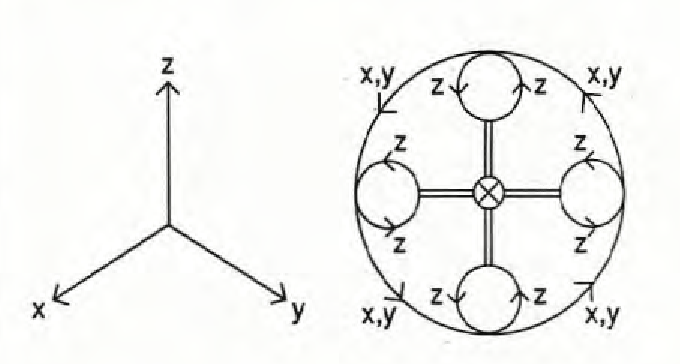
\includegraphics[width=0.3\textwidth]{./cycloid.png}\\[2cm]
\HRule \\[1cm]
{ \huge \bfseries Design of an Attitude and Heading Reference Sensor } \\[1cm]
\HRule \\[0.5cm]
{ \large \bfseries Presented for completion of an Independent Study in Electrical Engineering }
\\[0.5cm]
{ \large \bfseries Rutgers, The State University of New Jersey }
\\[0.5cm]
\HRule \\[1cm]

{\large Pat Hickey}
\\ 
pat@moreproductive.org
\\[0.5cm]
\emph{Advisor}
\\ Dr. Chung-chieh Shan
\\ Department of Computer Science
\vfill
{\large \today}

\end{center}
\end{titlepage}


\begin{abstract}
This paper describes the design of an Attitude and Heading Reference Sensor (AHRS), which measures rootational orientation relative to north and down. 
The design uses 3-axis accellerometer, magnetometer, and rate gyro sensors. 
I will discuss the selection and construction of the sensor hardware, design and implementation of a Kalman filter for sensor fusion, and the test of both the sensor hardware and software.
\end{abstract}


\section{Problem Description}

The goal of this project was to design and build sensor hardware and software that would determine the angular orientation and angular rotation rate of the sensor relative to the earth frame, ie. North, East, and Down. I selected sensor integrated circuits (ICs) which determine, on three axes, body accelleration, body rotation rate, and relative magnetic field. These three sensors (accellerometer, rate gyro, and magnetometer) provide a total of nine measurments. 

An algorithm is required to convert these nine measurments into an expression of angular orientation and angular rate (the derivative, with respect to time, of angular orientation). Angular orientation of a body has three degrees of freedom, as does angular rate. The conversion from measurment space to estimate space (a pair of angular orientation estimate and angular rate estimate) is nonlinear and uses a four-dimensional vector called a quaternion to describe the three-dimensional angular orientation. This is to say, a big part of the problem is ensuring the correctness of this difficult conversion process.   

I selected a well-known algorithm which implements a Quaternion Kalman Filter. This provides an state estimate using the four-dimensional quaternion vector, and an additional three-dimensional rotational rate vector. I needed to implement that software so that I could test it for correctness and use it to determine the orientation of an actual sensor. This software was to be used in an actual model aircraft autopilot system, so it must meet requirments for reliability and soft real-time performance.

\subsection{Application}

As part of my role on the Rutgers Autonomous Aircraft Team, I've been working on a model aircraft autopilot system based on a single board computer which runs Linux \footnote{For more information on this project, see \url{http://moreproductive.org/autopilot/}}. I implemented the control, navigation, and telemetry software in C using standard Linux system calls and threads. I used dedicated hardware for real-time tasks, for example, a microcontroller-based servo controller connected via USB ensures proper servo control despite irregular communication intervals from the computer. 
By using helper threads for input and output, we can be reasonably sure the main control loop will run at close to 60Hz. This is considered ``soft'' real-time.

The sensor software needs to cooperate with the soft real-time main control loop. In order to stabilize a fixed-wing aircraft, we need to update the main control loop's orientation estimate at at least 30Hz, preferably at 60Hz. So the sensor hardware must provide new measurments at a rate exceeding 30Hz, a complete measurment every 33ms. The sensor filtration software must complete computation in much less than a measurment period as not to dominate the CPU. Lets consider a target time of 500us per computation.

\subsection{Use of Haskell}

The sensor software I describe in this paper is typically implemented in a low level language such as C or C++ in order to give the programmer explicit control over memory allocation and input-output (IO) calls. In fact, open source implementations of functionally similar software is available. 

I decided to write the filter software using Haskell. Haskell is a purely functional language with a powerful type system, and is not typically used for soft real-time applications. However, I believe Haskell is well suited for writing algorithms because it can express mathematical concepts elegantly, and often transparently. It is often possible to reason about Haskell code in the exact same way as mathematics. This results in code which is code more readable and more easily modified. 

\section{Theoretical Basis}

The theoretical basis for this paper has been primarily drawn from -- cite dchoukrouns paper. I hope this section provides a clear explanation of how that theory applies to this project.

\subsection{Measurment Vectors}
Because the sensors are fixed to the frame (\emph{body}) we're estimating the orientation, accellerometer and magnetometer provide us with vector measurments in the body frame. We denote body frame vectors with $b_x$. The expecte vector of that measurment in the global frame is $g_x$. For example, the expected global frame accelleration $g_a = \begin{bmatrix} 0 & 0 & -1\end{bmatrix} $ in units normalized to $1g$ ($9.81m/s^2$)

By comparing a body frame vector to the global frame vector, we can find a rotation which transforms the global frame into the body frame. We call this the orientation estimate.  

\subsubsection{Accellerometer Measurment}

An accellerometer measures force exerted by a small test mass against a beam connected to the sensor body. The current generation of MEMS accellerometers uses etched silicon to build the test mass and beam structure, and measures the capicatance between the test mass and sensor body to determine the beam deflection. Since an accellerometer can only measure deflection, and therefore accelleration, in one direction, we use three separate sensors oriented to measure accelleration along three orthogonal axes. These three separate measured accellerations ($a_x, a_y, a_z$) can be considered as a three dimensional vector 
\begin{equation} \label{eq:defa}
  a = \begin{bmatrix}a_x&a_y&a_z \end{bmatrix}
\end{equation}

According to Newton's second law, $F = m a$ , the force on a body will be directly proportional to the accelleration of the body. When we consider a small test mass $m_t$ on a beam, and the system is at rest, the mass will exert a force $F_g = m_t g_b$, where $g$ is the accelleration due to gravity in the body frame. A body accelleration ab will exert a force $F_a = m_t a_b$. The sensor measures the sum of these two forces, so for any $F = F_g + F_a = m_t ( g_b + a_b )$. Because $m_t$ is constant, we can define the scaled measurment $a$ as 
\begin{equation} \label{eq:defza}
  a = \frac{F}{m_t} = g_b + a_b
\end{equation} 
 
In this application we're interesting in estimating $b_a$ in order to find the vector, in the body frame, which points straight down in the world frame. We include a measurment noise vector $\delta_a$, and find measurment $z_b$ as
\begin{equation} \label{eq:findgb}
  z_a = b_a + a_b + \delta_a
\end{equation}

On a body such as an aircraft, where accellerations $a_b$ may come from any direction at any time, we consider $a_b$ to be a zero-mean gaussian random vector with a covariance matrix 
\begin{equation} \label{eq:Qa}
  Q_a = \begin{pmatrix} \sigma_a^2 & 0 & 0 \\
	                      0 & \sigma_a^2 & 0 \\ 
	                      0 & 0 & \sigma_a^2 \end{pmatrix} 
\end{equation}

Covariance matrix $Q_a$ will be used in the measurment model of the Kalman Filter. We typically estimate a value for $\sigma_a$ to be between 2$g$ and 4$g$ for airborne applications. Since $\delta_a$ will be zero-mean and have a small variance compared to $a_b$ we can neglect it.

\subsubsection{Magnetometer Measurment}

A magnetometer measures the magnitude magnetic field in one direction. I refer the interested reader to ... for a physical explanation of magnetometer sensors. The three separate measured magnetic field magnitudes ($m_x, m_y, m_z$) are considered as a three dimensional vector
\begin{equation} \label{eq:defb}
  m = \begin{bmatrix} m_x & m_y & m_z \end{bmatrix}
\end{equation}

The measured magnetic field $z_m$ will be the sum of three vectors: the natural magnetic field of the earth in the body frame $b_m$, the magnetic field of the body $m_s$, and measurment noise $\delta_m$.
\begin{equation} \label{eq:zm}
  z_m = b_m + m_s + \delta_m
\end{equation}
In this filter we assume the magnetic field of the body $m_s$ to be constant\footnote{Electrical and mechanical components which emit a changing electromagnetic field, such as DC motors and switching power supplies, will cause trouble.}. We will estimate $m_s$ for the particular body the sensor is installed in. Measurment noise $\delta_m$ will be considered a zero-mean gaussian random vector with covariance matrix
\begin{equation} \label{eq:Qm}
  Q_m = \begin{pmatrix} \sigma_m^2 & 0 & 0 \\
	                      0 & \sigma_m^2 & 0 \\ 
	                      0 & 0 & \sigma_m^2 \end{pmatrix} 
\end{equation}

We will estimate $\sigma_m$ from a long sequence of samples taken with the filter hardware at rest.

The earth's magnetic field, in the global frame ($g_m$), will point towards magnetic north when projected onto a horizontal plane. (talk about magnetic field strength, magnetic declination angle here)


\subsubsection{Rate Gyro Measurment}

A rate gyro measures the rotation rate of a body about a single axis. We use three orthogonal rate gyros to estimate the rotational rate of the body, considered as a vector
\begin{equation} \label{eq:omega}
	\omega = \begin{bmatrix} \omega_x & \omega_y & \omega_z \end{bmatrix}
\end{equation}
The measurment $z_\omega$ can be considered as
\begin{equation} \label{eq:zomega}
	z_\omega = \omega + \Delta_\omega + \delta_\omega
\end{equation}
where rate gyro zero offset $\Delta_\omega$ is the constant vector output when the sensor body is at rest,
and measurment noise $\delta_\omega$ is a zero-mean gaussian random vector with covariance matrix
\begin{equation} \label{eq:Qomega}
	Q_\omega = \begin{pmatrix} \sigma_\omega^2 & 0 & 0 \\
	                  ]    0 & \sigma_\omega^2 & 0 \\ 
	                      0 & 0 & \sigma_\omega^2 \end{pmatrix} 
\end{equation}

In reality, zero offset $\Delta_\omega$ may drift with time and change in temperature. Compensation for this gyro drift is outside the scope of this paper, but has been solved in --cite dchokrouns better paper.

\subsection{Quaternion Representation}

There are a wide variety of resources which formally describe quaternions and their use in describing spatial rotations. I will give an overview of the most useful properties which will be used in this work.

A quaternion is a complex number with three imaginary components, $i,j,k$, which are defined such that $i^2 = j^2 = k^2 = ijk = -1$. Quaternions span a four-dimensional real-numbered space where a quaternion $a + b i + c j + d k$ can be considered as a vector $\begin{bmatrix}a & b & c & d \end{bmatrix}$. 

Quaternion multiplication is a noncommutative operation: $q_1 q_2$ is not equal to $q_2 q_1$ for all quaternions $q_1, q_2$. This property is useful because spatial rotation is a noncommutative operation as well.

The set of unit quaternions, all $q$ where $ ||q|| = 1$, are used to represent spatial rotations. For every unit quaternion $q$ 
there exists a unit vector $\mathbf{v} = \begin{bmatrix} v_x & v_y & v_z \end{bmatrix}, ||v|| = 1$ 
and an angle $\theta \in [-\pi, \pi]$ where 
$q = \begin{bmatrix} \cos (\theta/2) & v_x \sin (\theta/2) & v_y \sin (\theta/2) & v_z \sin (\theta/2)\end{bmatrix}$. The quaternion formed in this represents a spatial rotation about axis $\mathbf{v}$ of angle $\theta$. 
From this angle-axis notation, we can see that $q$ and $-q$ represent the same spatial rotation. 

The inverse quaternion $q^{-1} = a - bi - cj - dk$ of a unit quaternion $q$ represents the inverse rotation $q$. We can visualize this as the same angle of rotation $\theta$ about an inverted axis $\mathbf{v}$.

I refer the reader to --citations for more detailed information.

\section{Hardware}
\subsection{Sensors}
In order to simplify the design of the sensor module, I selected two digital ICs which contain all of the sensing elements and analog to digital interfaces onboard. 
Both digital devices selected require no external passive or active components aside from bypass capicators. Analog sensors, by comparison, often require several amplifier and filter components per channel, and often, for high resolution sensing applications, a discrete analog to digital converter (ADC) IC. In addition, analog ICs generally require an isolated ``quiet'' power and ground from digital ICs. 

\subsubsection{Three-axis Accellerometer and Magnetometer}
ST Micro's LSM303DLH, a three-axis accellerometer and magnetometer, was selected for this project. A single 6x6mm surface mount package contains both an accellerometer and magnetometer module, each with their own analog to digital converters and two-wire (I2C) serial interface. 

The three-axis accellerometer has a maximum range of ... and ... bits (... g) of resolution. The maximum sample rate is ... samples per second.

The accellerometer module includes a self-test functionality, which ...
I've implemented a boot time self-test in the embedded code.

The three-axis magnetometer has a maximum measurment range of  and ... bits (... unit) of resulution. The maximum sample rate is ... samples per second. 

The magnetometer module includes a self-test functionality, which ...
I've implemented a boot time self-test in the embedded code.

The LSM303DLH is presently (May 2010) unreleased by ST Micro. I would like to thank ST Micro for donating an evaluation board to my project. The evaluation board provided 0.1" pitch headers, and connected both the accellerometer and magnetometer module's I2C bus to a common pair of pins. It also provides a configurable interrupt output pin for both the accellerometer and magnetometer module. The board takes 3.3v power and ground.

% should include a photograph, citation

\subsubsection{Three-axis Rate Gyro}

Invensense's ITG-3200, a three-axis rate gyro, was selected for this project. A 4x4mm surface mount package contains three gyro axes, analog to digital converters, and a two-wire (I2C) serial interface. It has a full scale range of $\pm 2000$ degrees per second (deg/s) and 16 bits (14.375 LSB/deg/s) of resolution. The maximum sample rate is ... samples per second. Because the rate gyro is a MEMS device, it is important that the device is isolated from severe shocks, such as drops, which could cause internal damage.

The ITG-3200 was released by Invensense in April 2010 and is presently their flagship digital sensor. I would like to thank Invensense for donating an evaluation board to my project. The ITG-3200 was provided on an evaluation board with 0.1" pitch headers. It requires a pair of signals for I2C, an optional interrupt output signal, and 3.3v power and ground. The optional interrupt output signal can be configured to signal when an analog to digital conversion is complete.

% should include a photograph, citation

\subsection{Microcontroller}
A microcontroller was required to interface with the three sensor modules on a single I2C bus, perform boot-time configuration and self-test, and transfer measurments to a PC. I selected a Sparkfun Arduino Pro Mini board, a small 0.1" pitch pin header breakout board based on a 3.3v Atmel AtMega328 microcontroller. The AtMega328 provides a single UART and single I2C peripheral. 

The sensor board connects to the host computer with an FTDI serial to USB converter. The FTDI converter also provides 3.3v power to the board.

% should include a photograph, citation

\subsection{Construction}

Because each sensor evaluation board used 0.1" pitch pins, I was able to use a 0.1" pitch protoboard and female pin headers to build a prototype sensor. The assembled sensor prototype is 2.5" x 4.5" x 0.75" in outer dimensions. To prevent electrostatic discharge and physical damage, it is velcroed inside a protective cardboard box with a lining of stiff anti-static foam. 

% picture

A schematic drawing is provided in the appendix. % do this

\lstset{language=C++,basicstyle=\ttfamily}
\section{Embedded Software}
The code described in this section can be found at \url{http://github.com/pchickey/p4l-ahrs}. It is built using the open source Arduino IDE, which can be found at \url{http://arduino.cc}.

\subsection{Requirments}
The embedded software primarily needs to send the measurments read from the I2C bus to the host computer on its 
UART\footnote{Universal Asynchronous Receive and Transmit; the receive/transmit method used by many serial protocols including RS232} 
interface. Each sensor has a number of configuration registers which are accessed through the I2C interface which need to be 

\subsection{Sensor Communication}

The communication protocol for each sensor is best detailed in their datasheet, and I will not discuss them in depth here. The basic unit of interface is register read and register write. Some registers (for example, the latest measurment) are read-only, and reads may effect the state of the device. For example, a read of a register measurment on the ITG-3200 will clear the ``new measurment available'' flag on another register.   

Read Register and Write Register commands both block for nontrivial amounts of time.
\lstset{language=C++,basicstyle=\ttfamily}
From i2c\_registers.pde
\begin{lstlisting}
#include <Wire.h>
char i2cReadRegister(int i2c_device, char i2c_register)
{
  Wire.beginTransmission(i2c_device);
  Wire.send(i2c_register);
  Wire.endTransmission();
  Wire.requestFrom(i2c_device, 1);
  return Wire.receive();  
}

void i2cReadRegisterSequential(int i2c_device, char i2c_register, 
        int len, char * buf)
{
  Wire.beginTransmission(i2c_device);
  Wire.send(i2c_register);
  Wire.endTransmission();
  Wire.requestFrom(i2c_device, len);
  int ii;
  for(ii = 0; ii < len; ii++)
    buf[ii] = Wire.receive();
  return;
}
void i2cWriteRegister(int i2c_device, char i2c_register, char value)
{
  Wire.beginTransmission(i2c_device);
  Wire.send(i2c_register);
  Wire.send(value);
  Wire.endTransmission();
}  
\end{lstlisting}

The \lstinline$Wire$ library is provided by the Arduino IDE.  The \lstinline$Wire$ object is instantiated as the interface to the single I2C peripheral\footnote{For more information on the I2C bus, see ...} on the AtMega chip. The peripheral will control the bus state and provide byte-at-a-time synchronous transmit and receive. 

Note that \lstinline$beginTransmission(int)$, \lstinline$send(char)$, and \lstinline$requestFrom(int, int)$ only return after 8 bits have been sent on the I2C bus. At a bitrate of 100kHz we can expect this to take 80$\mu$s (0.08ms). A call to \lstinline$receive()$ will not return until one byte has been received on the bus. If the slave device responds immediately, this will only take 80$mu$s, but could possibly take longer if the slave device misbehaves and holds the bus in ``wait to receive'' state.
\begin{lstlisting}
void i2cWriteWithCheck(int i2c_device, char i2c_register, 
        char value, char* name)
{
  i2cWriteRegister(i2c_device, i2c_register, value);
  char check = i2cReadRegister(i2c_device, i2c_register);
  if (check != value)
  {
    Serial.print("$DEBUG,");
    Serial.print(name);
    Serial.print(" config appears unsuccessful.");
    Serial.print("expected ");
    Serial.print(int(value));
    Serial.print(" read ");
    Serial.println(int(check));
  }
}
\end{lstlisting}
In the boot configuration of sensors, I use a wrapper on \lstinline$i2cWriteRegister$ which confirms a write was successful. Unsuccessful writes usually indicate the sensor is malfunctioning.

% calculate best-case blocking time based on bus bitrate (100kbps?)

\subsection{Host Computer Communication}
A simple serial protocol, based on NMEA-style sentences (cite), is defined for communication with the host computer. 

\subsection{Arduino Environment}
The Arduino environment is an IDE, C/C++ compiler, and collection of libraries for AtMega328 and similar Atmel AVR microcontrollers. It provides a high level interface to the hardware and is suitable for rapid prototype development. 

The timing and logic requirments of the I2C and UART interfaces are handled in hardware, and the Arduino environment provides a library for blocking read and write operations on both of these interfaces. 

On reset\footnote{The most common way to program AVR and similar microcontrollers is unsupervised by any kernel, therefore ``bare metal''. Essentially, on power on a bootloader checks for new firmware over the serial port, and if none is found, passes control to a single entry point. The C linker will choose \lstinline$main()$ unless told otherwise. This bare metal code can only be superceded by interrupt service routines.}
, the Arduino environment will intitialize and call \lstinline$void setup()$. This code runs once and should setup all of the interfaces which will remain the same throughout execution. The setup code then initializes the configuration registers of the sensor devices, performs sanity checks of those registers to ensure successful writes, and performs the self-test of the magnetometer and accellerometer device. 

% listing here

Once the \lstinline$setup$ routine has returned, the Arduino environment will call \lstinline$void loop()$ in an endless loop. This code performs reads of any available sensor measurment, and prints the result to the serial port.

% listing here

In this code, many operations involve serial reads and writes which block for significant amounts of time. The (... check new) calls actually read registers on the sensor device, which takes a nontrivial amount of time. 



describe arduino programming environment
blocking serial calls
-- Provide timing information?

\section{Filtration Software}
The filtration software was implemented in Haskell. The code may be found on Github at \url{http://github.com/pchickey/hs-qkf/}
\lstset{language=Haskell}
\subsection{Algorithm Selection}
I based the algorithm of Daniel Choukroun's "A Novel Quaternion Kalman Filter" (cite). The paper defines an algorithm for using both vector (accellerometer and magnetometer) and derivative (rate gyro) measurments optimally. Notably, it updates a quaternion state estimate by finding a Kalman filter observation matrix $H$ which relates body-frame vector measurments to the rotational frame estimate.

I used James Deibel's "..." (cite) as a reference source for converting angular representations of orientation to quaternion representions, and vice versa. 

\subsection{Implementation of Filter}

\subsubsection{Quaternion.hs}
I define the \lstinline$Quat$ type in a module which is used by several others. This provides standard accessors, mapping quaternion components names to their element as a \lstinline$Vector D4 Double$.
\begin{lstlisting}
module Quaternion where
import Numeric.LinearAlgebra.Static
type Quat = Vector D4 Double

-- Quaternion accessor convention:
-- In the James Deibel paper, quaternions 
--    are [re i j k] ordered; 
-- type Quat used by module Qkf is [i j k re] ordered.
-- Therefore, use these accessors for the 
--   component within this program

-- Real component
q0 :: Quat -> Double
q0 = (@>3) 
-- i component
q1 :: Quat -> Double
q1 = (@>0)
-- j component
q2 :: Quat -> Double
q2 = (@>1) 
-- k component
q3 :: Quat -> Double
q3 = (@>2) 
\end{lstlisting}

\subsubsection{Qkf.hs}
The quaternion Kalman filter is implemented in a single haskell module.
\begin{lstlisting}

module Qkf where
-- 9 out of 10 computer scientists recommend hmatrix-static
import Numeric.LinearAlgebra.Static
import Quaternion
\end{lstlisting}


The \lstinline$Numeric.LinearAlgebra.Static$ module, distributed on hackage as \emph{hmatrix-static}\footnote{\url{http://hackage.haskell.org/package/hmatrix-static}. N.B. hmatrix-static 0.3 is only compatible with ghc-6.10 at the time of this writing.}, 
is a matrix library which makes it possible to type-check matrix operations based on the dimensions of their operands at compile time. This helps ensure code correctness and eliminates a subset of runtime errors.

The \lstinline$Quaternion$ module has been defined above.

\begin{lstlisting}
-- for deltaT and so on
type Time = Double
-- vec first {i j k}, then re
type QuatCovMat = Matrix (D4, D4) Double
-- Defined in paper, but we don't use it?
type AttitudeMat = Matrix (D3, D3) Double
-- All 3-space Measurments are zero-mean
type MeasurmentCovMat = Matrix (D3, D3) Double
type RateCovMat = Matrix (D3, D3) Double
-- 3-space vectors for acc,mag
type BodyVec = Vector D3 Double
type RefVec = Vector D3 Double
-- 3-space angular rate, measured in Body frame
type AngularRate = Vector D3 Double
-- Observations are of form 0 = Hnot*q
type ObservationMat = Matrix (D4,D4) Double
-- Observation noise maps 3space to quat space
type ZetaMat = Matrix (D4,D3) Double
-- Translate qspace to qspace
type TransitionMat = Matrix (D4,D4) Double

\end{lstlisting}

I define types for every particular matrix and vector used in the filter. This makes code more readable because the type signature is more specific. 

\begin{lstlisting}
data FilterState = 
  FilterState{ q :: Quat
             , p :: QuatCovMat } deriving( Show, Eq )

data RateEstimate = 
  RateEstimate{ omega   :: AngularRate
              , qke :: RateCovMat
              , dt      :: Time } deriving( Show, Eq )

data MeasurmentSource = Accelerometer
                      | Magnetometer 
                      | Gyro deriving( Show, Eq )

data Measurment =
  Measurment{ source  :: MeasurmentSource
            , body    :: BodyVec
            , ref     :: RefVec
            , meascov :: MeasurmentCovMat } deriving( Show, Eq )


\end{lstlisting}

Datatypes are defined for information which is temporally associated.

\begin{lstlisting}

qzero :: Quat
qzero = [$vec| 0, 0, 0, 1|]

-- [ex]; Cross-product matrix of 3x1 column vector e, defined as
crossProdMat :: (Element a) => Vector D3 a -> Matrix (D3,D3) a
crossProdMat v = 
  [$mat| 0, -1*e3, e2 
       ; e3, 0, -1*e1 
       ; -1*e2, e1, 0 |]
  where 
  e1 = v @> 0
  e2 = v @> 1
  e3 = v @> 2

\end{lstlisting}

The \lstinline& [$mat| |] & and \lstinline& [$vec| |] & macros make it possible to construct matricies and vectors in a similar syntax to Matlab, which greatly aids readability.

\begin{lstlisting}

qre :: Quat -> Double
qre q = q @> 3

qvec :: Quat -> Vector D3 Double
qvec q = 
  [$vec| q0, q1, q2 |]
  where 
  q0 = q @> 0
  q1 = q @> 1
  q2 = q @> 2

\end{lstlisting}
The \lstinline$qre$ and \lstinline$qvec$ accessors provide a syntax that resembles that in D. Choukroun's paper.
\begin{lstlisting}
unitq :: Quat -> Quat 
unitq qq = 
  qq / constant norm 
  where 
  norm = sqrt $ (qq@>0)*(qq@>0)+(qq@>1)*(qq@>1)+
		(qq@>2)*(qq@>2)+(qq@>3)*(qq@>3)

\end{lstlisting}

Some quaternion manipulations in the Kalman filter do not produce a unit quaternion because D. Choukroun's derivations did not require unit length. To simplify the interface to the filter, we normalize a quaternion with \lstinline$unitq$.

\begin{lstlisting}
attMatOfQ :: Quat -> AttitudeMat
attMatOfQ qq = 
  liftMatrix (*constant  (q*q - e <.> e)) (ident `atRows` d3) + 
  liftMatrix (*constant 2)  (outer e e) -
  liftMatrix (*constant (2*q)) (crossProdMat e)
  where 
  q = qre qq 
  e = qvec qq

-- mulQLeftMat is the matrix Q1 of q1 where 
-- Q1<>q2 = quaternion multiplication q1*q2
mulQLeftMat :: Quat -> Matrix (D4, D4) Double
mulQLeftMat qq = [$mat| w, -z,  y,  x;
                        z,  w, -x,  y;
                       -y,  x,  w,  z;
                       -x, -y, -z,  w|]
  where w = qq @> 3; x = qq @> 0; y = qq @> 1; z = qq @> 2

-- quaternion multiplication
mulqq :: Quat -> Quat -> Quat
mulqq q1 q2 = (mulQLeftMat q1) <> q2

-- inverse quaternion: negate the axis to 
-- reverse direction of rotation
invq :: Quat -> Quat
invq qq = [$vec| -x, -y, -z, w |]
  where w = qq @> 3; x = qq @> 0; y = qq @> 1; z = qq @> 2

rad2deg :: (Floating a) => a -> a
rad2deg rads = rads * 180.0 / pi
deg2rad :: (Floating a) => a -> a
deg2rad degs = degs * pi / 180.0

\end{lstlisting}

Utility functions that should be self explanatory.

\begin{lstlisting}
-- The vecQ functions are for rotating a 
-- three-space vector by a quaternion
vecQRightMat :: Vector D3 Double -> Matrix (D4, D4) Double
vecQRightMat b = 
  ((negboX <|> bo) <-> (negbot <|> [$mat| 0 |]))
  where 
  negboX = liftMatrix (*constant (-1)) (crossProdMat b)
  bo = asColumn b
  negbot = liftMatrix (*constant (-1)) (asRow b)

vecQLeftMat :: Vector D3 Double -> Matrix (D4, D4) Double
vecQLeftMat b = 
  ((boX <|> bo) <-> (negbot <|> [$mat| 0 |]))
  where 
  boX = crossProdMat b
  bo = asColumn b
  negbot = liftMatrix (*constant (-1)) (asRow b)
\end{lstlisting}

Hmatrix-static provides operators \lstinline$<->$ and \lstinline$<|>$ to join matricies horizontally and vertically.

\begin{lstlisting}
observationMatOf :: RefVec -> BodyVec -> ObservationMat
observationMatOf r b = 
  ( (negsx <|> asColumn d) <->
    (negdt <|> [$mat|0|]) )
  where 
  s = liftVector2 (*) (constant 0.5) (b + r)
  d = liftVector2 (*) (constant 0.5) (b - r)
  negsx = liftMatrix (*constant (-1)) (crossProdMat s)
  negdt = liftMatrix (*constant (-1)) (asRow d)
\end{lstlisting}

The observation matrix (in ..., $H$) is a function of the measurment BodyVec and known RefVec.

\begin{lstlisting}
zetaMatOf :: Quat -> ZetaMat
zetaMatOf qq = 
  (ex + liftMatrix (* constant q) (ident `atRows` d3)) <-> 
  (liftMatrix (* constant (-1)) (asRow e))
  where 
  q = qre qq
  e = qvec qq
  ex = crossProdMat e

\end{lstlisting}

The matrix $\Xi$, which I ignorantly coded as ``Zeta,'' maps measurment error into the state space in the same way the matrix $H$ maps measurments into the state space.

\begin{lstlisting}
transitionMatOf :: AngularRate -> Time -> TransitionMat
transitionMatOf w dt = 
  expm omegadt
  where 
  omega = vecQRightMat w
  omegadt = liftMatrix (* constant dt) omega

\end{lstlisting}

This transition matrix is derived in ... as a matrix multiplication on a quaternion. I wanted to ensure it was equivelant to the more common derivation, and so I wrote a function below, \lstinline$transitionQuatOf$, which uses quaternion multiplication and the angle-axis method.

\begin{lstlisting}

transitionQuatOf :: AngularRate -> Time -> Quat
transitionQuatOf w dt = 
  [$vec| qx, qy, qz, qre |]
  where
  wx = w @> 0; wy = w @> 1; wz = w @> 2
  qx = sin $ wx * dt
  qy = sin $ wy * dt
  qz = sin $ wz * dt
  qre = 1 - (qx*qx + qy*qy + qz*qz)

timePropogate :: RateEstimate -> FilterState -> FilterState
timePropogate r s = 
  FilterState { q = unitq $ phi <> (q s)
              , p = phi <> (p s) <> (trans phi) + qkq }
  where 
  phi = transitionMatOf (omega r) (dt r)
  zeta = zetaMatOf (q s)
  zetat = ((dt r)/2)^2
  qkq = liftMatrix (*constant zetat) (zeta <> (qke r) <> (trans zeta))

timePropogate' :: RateEstimate -> FilterState -> FilterState
timePropogate' r s = 
  FilterState { q = mulqq qomega (q s)
              , p = phi <> (p s) <> (trans phi) + qkq }
  where 
  qomega = transitionQuatOf (omega r) (dt r)
  phi = transitionMatOf (omega r) (dt r)
  zeta = zetaMatOf (q s)
  zetat = (^2) . (/2) . dt $ r
  qkq = liftMatrix (*constant zetat) (zeta <> (qke r) <> (trans zeta))  

\end{lstlisting}
Two similar versions of timePropogate, the second explicitly using quaternion multiplication for propogation. This is an example which demonstrates how simple it is to modify an algorithm in Haskell.

\begin{lstlisting}

measurmentUpdate :: Measurment -> FilterState -> FilterState
measurmentUpdate m s = 
  FilterState { q = unitq $ up <> (q s)
              , p = up <> (p s) <> (trans up) +
                    k <> rq <> (trans k) }
  where 
  i4 = ident `atRows` d4
  alpha = 0.001
  h = observationMatOf (ref m) (body m)
  ht = (trans h)
  zeta = zetaMatOf (q s)
  rq = (liftMatrix (*constant 0.25) 
           (zeta <> (meascov m) <> (trans zeta))) + 
       (liftMatrix (*constant alpha) i4)
  sk = h <> (p s) <> ht + rq 
  k = (p s) <> ht <> (inv sk)  
  up = (i4 - k <> h)

\end{lstlisting}
A measurment update maps FilterState to FilterState with a Measurment. If that doesn't make nice semantic sense, I don't know what does. 

\begin{lstlisting}

rateEstimateUpdate :: Measurment -> Time -> RateEstimate -> RateEstimate
rateEstimateUpdate Measurment { source = Gyro, body = b } adt re = 
  RateEstimate { omega = (omega re) + constant k * residual
               , qke = (qke re)
               , dt = adt }
  where 
  k = 0.3
  residual = b - (omega re)

rateEstimateUpdate _ _ re = re 

-- rezero: initial state for rate estimate. 
rezero = RateEstimate { omega = [$vec|0,0,0|]
                      , dt = 0.02
                      , qke = liftMatrix (*constant 10) (atRows ident d3) }
fszero = FilterState { q = qzero
                     -- p is large to account for random initial position
                     , p = liftMatrix (*constant 5) (atRows ident d4) }

fnorm x = pnorm PNorm2 x
\end{lstlisting}
I provide initialized filter states in this module as well, with constants that were found to be appropriate.

\subsection{Implementation of Tests}
In order to test the quaternion Kalman filter, I wrote some Euler angle translation functions using ... in order to visualize simple rotational frames. The Euler angles have various issues that prevent them from being useful to describe filter state, the most significant of which is the condition called \emph{gimbal lock} where, at``poles'' in the spherical space, it is impossible to determine one of the three angles. An analogy of this problem using the earth's geography as a spherical space is that, from the north pole, each direction is south, and the directions of east and west cannot be determined.

\begin{lstlisting}
{-# LANGUAGE QuasiQuotes #-}
module Eulers321 where

import Numeric.LinearAlgebra.Static
import Quaternion

type Angle = Double
type RotMatrix = Matrix (D3,D3) Double
type Eulers = Vector D3 Double
type WorldAngularRate = Vector D3 Double
-- ordering is [phi, theta psi] naturally
phi :: Eulers -> Angle
phi e = e @> 0
theta :: Eulers -> Angle
theta e = e @> 1
psi :: Eulers -> Angle
psi e = e @> 2
-- For convenience:
ezero :: Eulers
ezero = [$vec|0,0,0|]

-- Make a rotation matrix from Euler angles. Deibel (449)
matOfEulers :: Eulers -> RotMatrix
matOfEulers eulers = 
  [$mat| cphi*cthe , sphi*cpsi + cphi*sthe*spsi , sphi*spsi - cphi*sthe*cpsi 
       ;-sphi*cthe , cphi*cpsi - sphi*sthe*spsi , cphi*spsi + sphi*sthe*cpsi
       ;  sthe     ,-spsi*cthe                  , cpsi*cthe                  |]
  where
  cphi = cos . phi   $ eulers
  sphi = sin . phi   $ eulers
  cthe = cos . theta $ eulers
  sthe = sin . theta $ eulers
  cpsi = cos . psi   $ eulers
  spsi = sin . psi   $ eulers

-- Make a quaternion from Euler angles. Deibel (459),
--  except re-ordered with real component last
-- to fit type Quat convention.
qOfEulers :: Eulers -> Quat
qOfEulers eulers =
  [$vec| 
         cphi * cthe * spsi + sphi * cpsi * sthe,
         cphi * cpsi * sthe - sphi * cthe * spsi,
         cphi * sthe * spsi + cthe * cpsi * sphi,
         cphi * cthe * cpsi - sphi * sthe * spsi
         |]
  where
  cphi = cos . (/2) . phi   $ eulers
  sphi = sin . (/2) . phi   $ eulers
  cthe = cos . (/2) . theta $ eulers
  sthe = sin . (/2) . theta $ eulers
  cpsi = cos . (/2) . psi   $ eulers
  spsi = sin . (/2) . psi   $ eulers

-- Deibel (452)
eulersOfQ :: Quat -> Eulers
eulersOfQ q =
  [$vec| atan2 ((-2)*qq1*qq2 + 2*qq0*qq3) 
               (qq1*qq1 + qq0*qq0 - qq3*qq3 - qq2*qq2)
       , asinLimited (2*qq1*qq3 + 2*qq0*qq2)
       , atan2 ((-2)*qq2*qq3 + 2*qq0*qq1) 
               (qq3*qq3 - qq2*qq2 - qq1*qq1 + qq0*qq0) |]
  where 
  qq0 = q0 q; qq1 = q1 q; qq2 = q2 q; qq3 = q3 q
  asinLimited x = if (abs x) < 1.0 
                    then asin x 
                    else asin (signum x) 
              -- v small numeric overflows: 
              -- keep args to asin in [-1,1]

-- Euler Angle Rate Matrix
-- omega = E(u) * udot  where omega is body fixed angular rates, u is euler angles
-- Deibel (453)
type Emat = Matrix (D3,D3) Double
-- Deibel (453)
ematOfEulers :: Eulers -> Emat
ematOfEulers e = [$mat| sthe      , 0    , 1
                      ;-spsi*cthe , cpsi , 0
                      ; cpsi*cthe , spsi , 0 |]
  where
  cthe = cos . theta $ e
  sthe = sin . theta $ e
  cpsi = cos . psi   $ e
  spsi = sin . psi   $ e


\end{lstlisting}

We use this notation in 
rotation-matrix based vector measurment simulation
addition of noise
\subsection{Sensor Interface}
serial.hs
\subsection{Gnuplot Interface}
overview, code snippets
\subsection{OpenGL Demonstration Interface}
cube.hs overview, code snippets 
\subsection{Paparazzi Autopilot Interface}
ffi, linux mq
"ongoing investigation" is code for, I haven't done it yet

\section{Results}
\subsection{Noise-free simulated measurments}
Plots of step test, ramp test
\subsection{Noisy simulated measurments}
step test, ramp test
\subsection{Tests with Sensor}
plots, link to video on youtube

\end{document}


